\chapter{Restricciones y Cotas}

\begin{figure}[H]
	\centering
	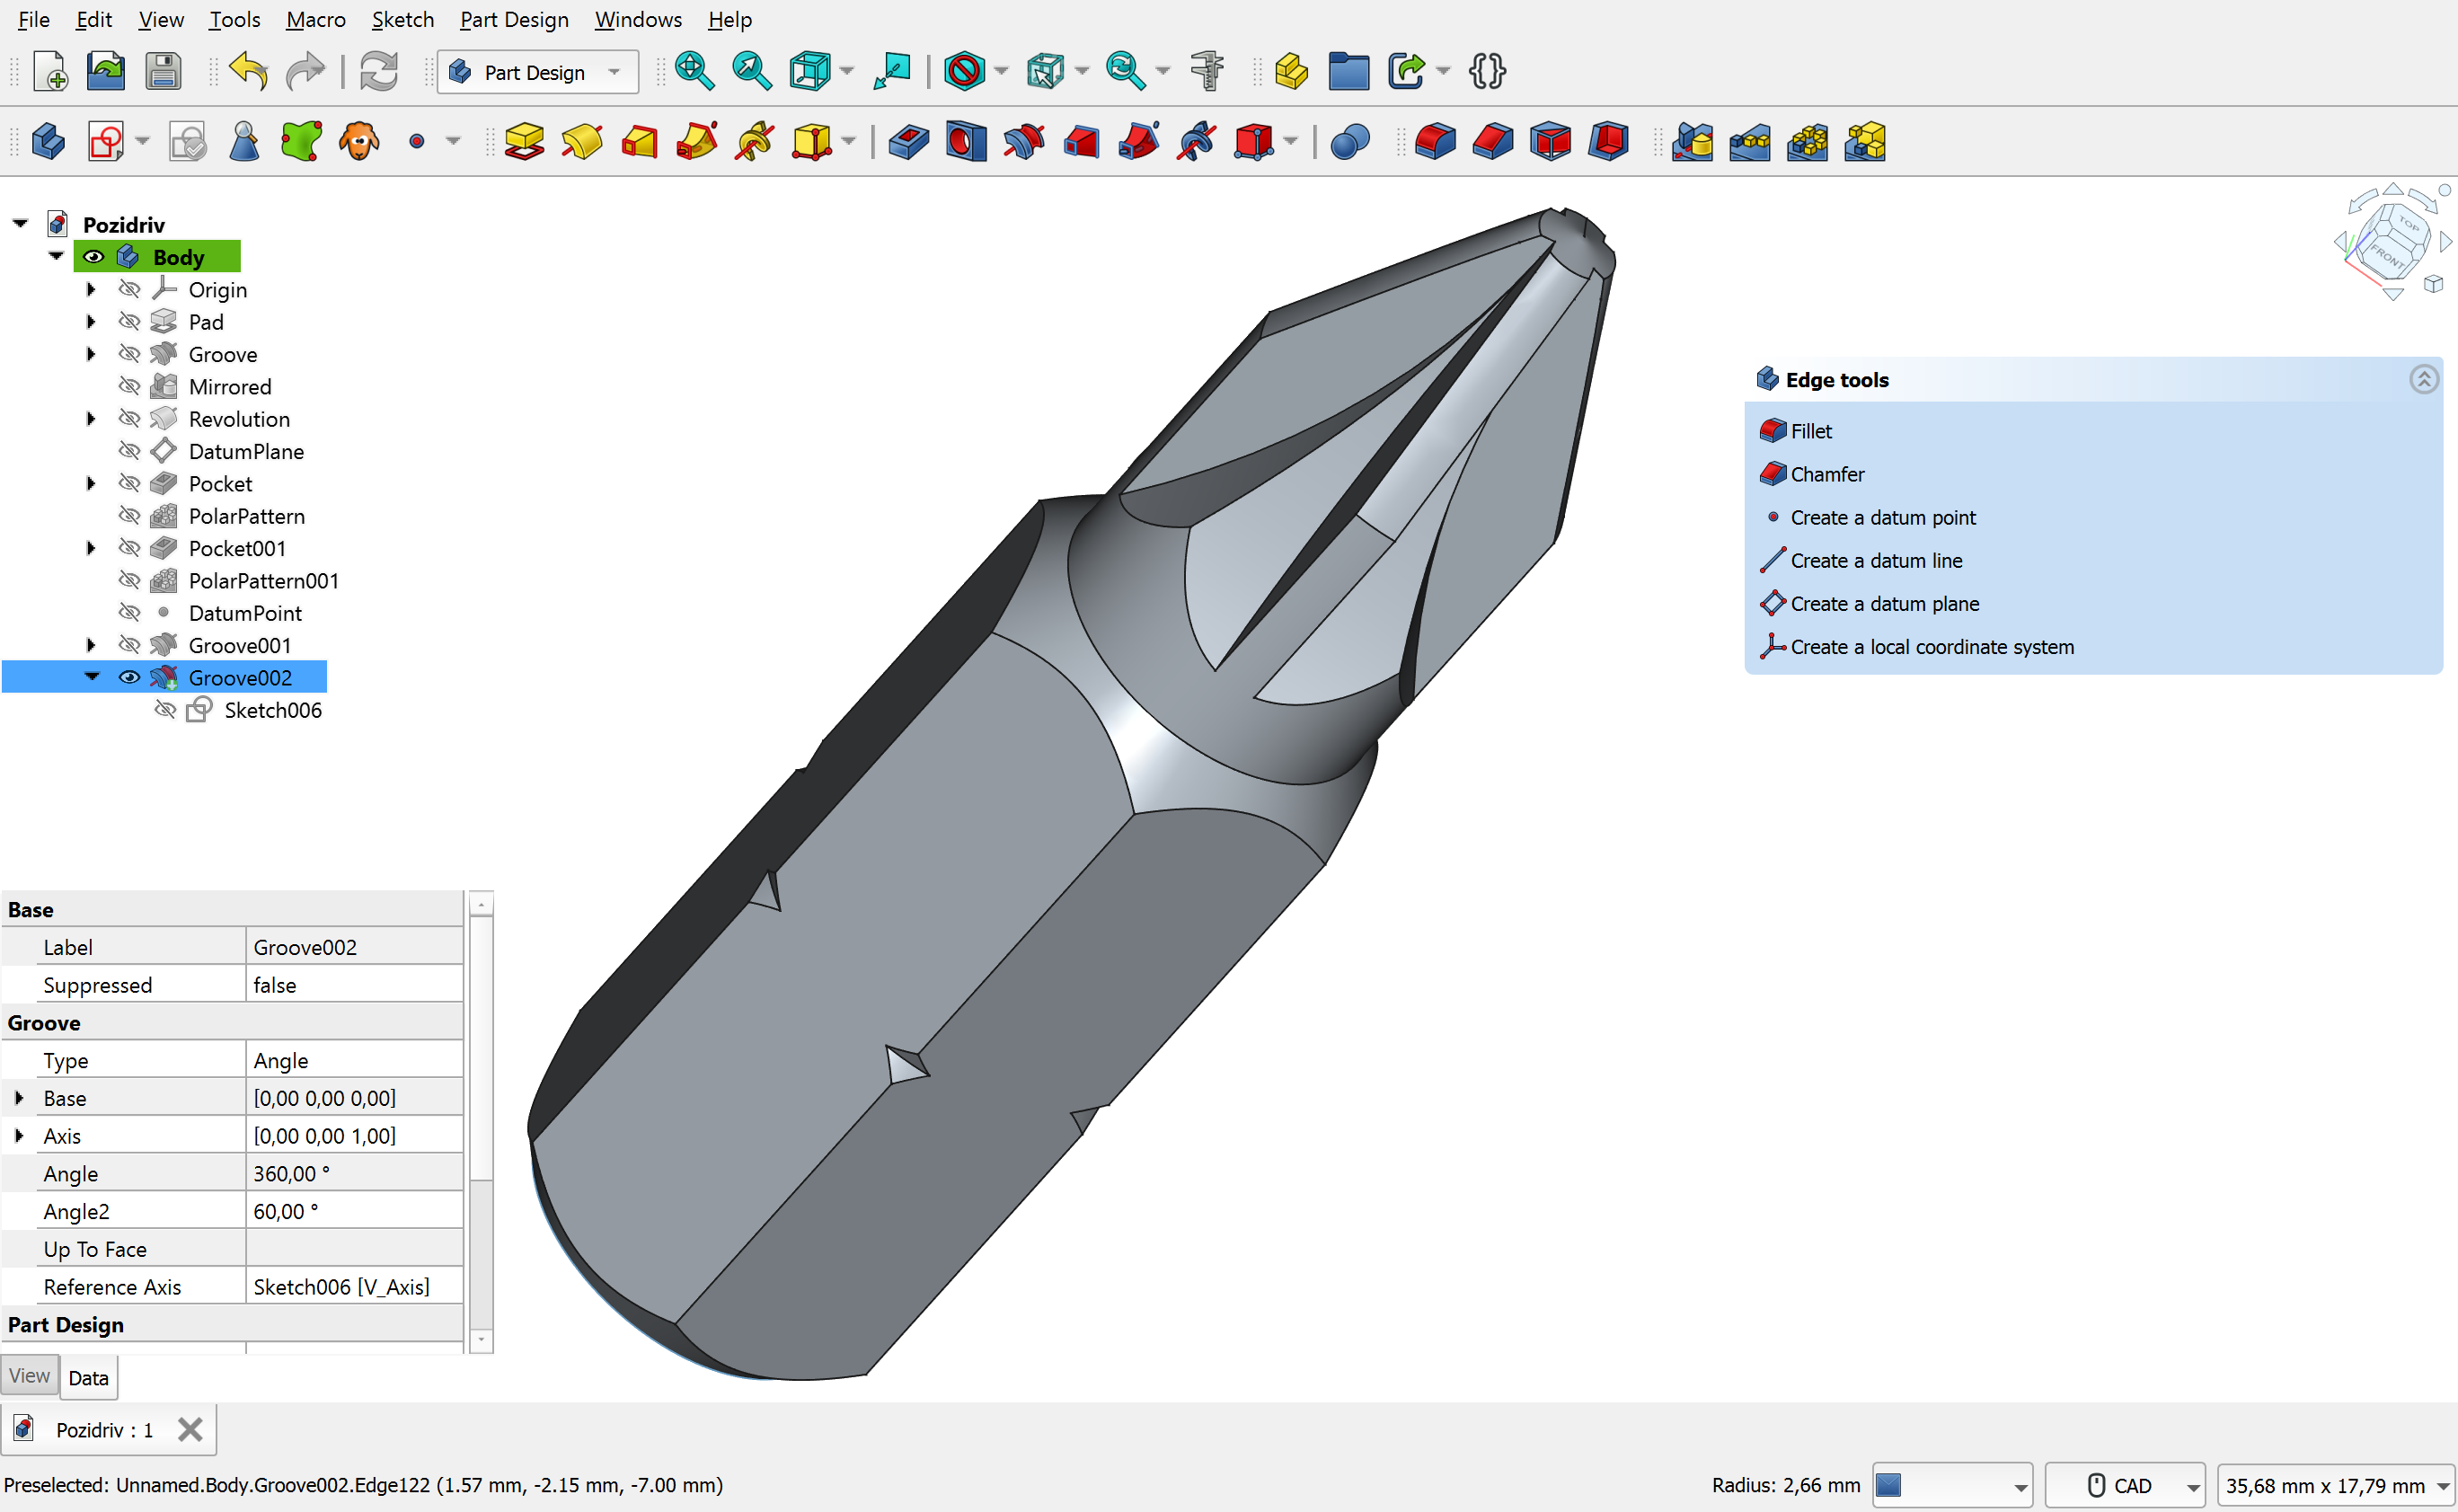
\includegraphics[width=0.8\textwidth]{img/cap5_restricciones.png}
	\caption{Boceto con restricciones geométricas y dimensionales}
\end{figure}

Aprende a aplicar restricciones geométricas y cotas
dimensionales a tus bocetos. El control preciso de
dimensiones es fundamental en diseño paramétrico.

%% D. Búsqueda e Inserción de Activos Gráficos
%% Imagen insertada al inicio del capítulo

%% B. Actividades Teóricas
\section{Investigar y responder}
\faPencil

Investiga sobre restricciones en FreeCAD y responde:
\begin{enumerate}
	\item ¿Qué son las restricciones geométricas en un
	      boceto?
	\item ¿Cuál es la diferencia entre restricciones
	      geométricas y dimensionales?
	\item ¿Qué restricciones se aplican a líneas paralelas
	      y perpendiculares?
	\item ¿Cómo se fijan longitudes y ángulos exactos?
	\item ¿Qué es una cota y cómo se edita?
	\item ¿Qué significa ``fully constrained'' en un boceto?
	\item ¿Cómo se aplican restricciones de simetría?
	\item ¿Qué errores comunes ocurren al aplicar
	      restricciones?
\end{enumerate}

%% C. Actividades Prácticas
\section{Resolver los siguientes problemas}
\faWrench

Problemas para aplicar conocimientos:
\begin{enumerate}
	\item Crea un rectángulo con restricciones de igual
	      longitud en los lados opuestos.
	\item Dibuja dos líneas paralelas y aplica restricción
	      de distancia entre ellas.
	\item Crea un triángulo con restricciones de igual
	      longitud en los tres lados.
	\item Dibuja un círculo inscrito en un cuadrado usando
	      restricciones de tangencia.
	\item Crea una figura con restricciones de perpendicularidad
	      entre líneas.
	\item Aplica restricciones de simetría a una figura
	      respecto a un eje.
	\item Modifica las cotas de un boceto existente y
	      observa cómo cambia la forma.
	\item Crea un boceto completamente restringido de una
	      pieza mecánica simple.
	\item Identifica y corrige restricciones conflictivas
	      en un boceto.
	\item Practica la edición masiva de cotas en un boceto
	      complejo.
\end{enumerate}